\part{古典经济思想及其批判}

通常所说的经济学古典时期,涵盖了一百多年的经济思想,其方向与主要贡献者几乎为英国
人所垄断。

从1776年到1820年几乎是斯密时代,从大约1820年到19世纪50年代是李嘉图时代,从19世纪
50年代到19世纪90年代是约翰·斯图亚特·穆勒时代。

另外两位先行思想家是马尔萨斯与马克思,尽管他们在某些方面来看属于古典学派,但是与
作为古典经济学的拥护者相比,他们作为古典经济学批评家的意义更大。马尔萨斯的人口理
论符合古典理论,但是马尔萨斯在他对经济体某些宏观方面的分析中,以及在他对地主阶层
的作用与重要性的捍卫中,却引人注目地背离了正统的古典传统。但是,我们将单独考察马
尔萨斯与李嘉图之间关于经济体自动实现资源充分利用的著名论战。卡尔·马克思从古典经
济学中汲取了一些因素,加入了不同的看法和一些新的分析概念,得出了与古典理论及政策
直接相对立的结论。

\subsection*{古典政治经济学}
\addcontentsline{toc}{subsection}{古典政治经济学}

与重商主义思想最大的不同是,他们对经济力量自然运作所产生的结果持赞同态度。在古典
经济学家眼里,经济体制通常是和谐的,这与重商主义者与经院哲学的信仰尖锐对立,重商
主义者与经院哲学均认为市场的特征在于不和谐,需要进行限制和干预。

法国重农主义者最早引人注目地提出了下面的观点,即针对相对稀缺性产生的冲突,市场自
动地提供和谐的解决办法……政府应当对经济体采用自由放任的政策……

古典学派确信借助自由这一手段,经济体能够最有效率地运行。他们断言,个人与厂商应当
不受政府干预地自由交易。除此之外,古典学派认识到,政治自由与经济自由是不可分割地
绑在一起的,亮着彼此影响。

但他们也非常了解社会冲突,尤其是地主与那些提倡经济增长与变革,并从中获益的人之间
的冲突。正像斯密与李嘉图两人所理解的那样,资本主义的长期趋势导致了这些不和谐的后
果。

经济体制中和谐概念相关的两条显著的发展路径。一方面是,主流正统经济思想尽管一直不
断地接受和谐运行的经济体制这一基本前提,却正通过越来越多地鼓吹经济问题的政治反应
而非经济反应,缓慢而稳定地弱化这一前提。另一方面,一些非主流经济学家否认古典经济
学所认同的和谐性,并发现了体制中的一些基本冲突,这些冲突需要对制度结构进行主要变
革才能加以解决。马克思主义思想是下面这种经济思想最重要的例子,即认为经济体制充满
了矛盾冲突,通过市场力量无法予以解决。

古典经济学派的第二个特征是它对经济增长的关注。……宏观……所以古典经济学家致力于
发掘决定经济增长率的力量、文化、政治、社会、历史因素。这方面凯恩斯主义者的主要关
注点是决定经济活动水平的力量。他们考虑某一时点上一个经济体是否在低于资源充分利用
的水平上运用。古典经济学派对这一问题并不感兴趣,因为他们已经假设经济体倾向于在资
源充分利用的水平上运行。当现代宏观经济学背离凯恩斯主义宏观经济学时,又回到了这些
相同的问题与假设上来,所以,现代宏观经济学家有时也被称为“新古典经济学家”。

古典经济学家对增长的关注使得他们去研究市场,研究作为资源配置者的价格体制。……古
典学派延续了重商主义者的传统,因为两者都聚焦于我们今天所谓的“宏观经济学”。

相比古典经济学,新古典经济学在比较静态的框架中研究市场,目的是使下面的这些问题更
加清楚,即什么力量决定了相对价格,生产了什么种类与数量的消费者产品,利用了什么种
类与规模的经济计划,收入的个人分配与功能分配是如何决定的。直到19世纪70年代,初生
的新古典经济理论才将经济学家的注意力从增长上引开,几乎专门研究有关在供选择的用途
之间分配稀缺资源的微观经济问题。

斯密经济学的最后一个统一特征代表了与重商主义思想的显著背离。尽管重商主义者的理论
结构是不牢固的,但是他们相信自己有能力了解经济体的运行。一旦他们认为自己获得了这
方面的知识,就会认为对他们所洞察的经济体运行中的任何缺陷进行修补是合适的。这种修
补要么通过变更制度结构,要么通过允许政府干预来实现。……重商主义者的角色认知与亚
当·斯密的怀疑论完全相对,斯密向胆敢以其判断来替代市场判断的政治家贤人提出了质疑。

\subsection*{马克思的政治经济学}
\addcontentsline{toc}{subsection}{马克思的政治经济学}

卡尔·马克思是古典经济学最重要的批评家,也是打造古典(classical)一词的人。马克思
是经济思想史的学生……影响马克思的最重要的经济学家是李嘉图。尽管古典经济学派发现
经济体是基本和谐的,并因此提倡自由放任的政府政策,但他们同时也发现了很多冲突。其
中之一就是地主与资本家之间的冲突。马克思指向资本家与劳动者之间的经济冲突。他改造
了古典学派的劳动价值理论以支持他的观点,即劳动者受到资本家的剥削。

古典经济理论与新古典理论不同,其分析的事物与结构是动态的。亚当·斯密集中研究经济
增长,大卫·李嘉图对资本主义中发生的收入分配的长期变化感兴趣。马克思的经济分析只
是其兴趣点的一部分,他的兴趣点是引起历史变革的力量。然而,古典学派所研究的一些相
同的动态问题,也引起了马克思的兴趣,例如,随着时间的变化,收入分配发生怎样的变化,
利润率将采取怎样的进程,大众福利水平的前景如何。

李嘉图和马克思都对劳动价值论感兴趣,但并不是因为它解释了某一时点上什么力量决定了
相对价格,也不是因为它把在可替代的用途之间有效分配稀缺资源的问题说得更清楚。马克
思想表明,剥削是如何根植于劳动者不拥有生产手段的体制中的;李嘉图则运用劳动价值论
来解释随着时间的变化收入分配的变化。

马克思对古典经济学的另一借鉴:对古典学派来说,主要的参与者是资本家、地主、劳动者。
在某种意义上,古典理论是对经济运行和对这些阶级的未来的一种分析。古典学派与马克思
都将社会中的动态因素视为资本家阶级活动的结果。

古典学派与马克思之间的差异比他们的相似之处更加显著,他们之间最重要的分歧是相互抵
触的意识形态上的观点。古典学派发现,资本家的利润动机导致经济体中资本的有效配置,
并导致储蓄,这将促进经济的增长和财富的增加。马克思则将资本家的活动看做是最终有害
于无产阶级和社会的。

\chapter{亚当·斯密}

\section{亚当·斯密的博学多才}

经济学家、大学教师。私密讲授一系列课程,其中包括我们现在所称的社会科学与人类学,他
主要对道德哲学感兴趣。他注意到经济自由与政治自由之间的重要关系,私人财产权利与公
正状态之间的重要关系,以及由利己主义所推动的个体与由关注其行为对他人产生的后果所
推动的个体之间的重要关系。

曼德维尔的讽刺风格令其对重商主义立场的表述广为流行。曼德维尔与斯密都是从人类利己
本性这一相同的假设出发,但却得出了相反的结论。曼德维尔主张,个人对私利的追求,会
产生很多不良的社会和经济后果,因此他为政府干预经济构建了一个实例。

斯密所处的时代,已有的不同研究领域之间不存在清晰的界定:哲学、自然科学、社会科学、
道德都被当做真理统一体的不同方面来对待,而不是当做单独的学科。此外,从事研究的知
识精英受到了严格意义上的教育,他们被要求掌握最宽广的人类知识。

这种多学科方法的一个后果是,那些像亚当·斯密一样,主要探求我们现在称为社会科学与
道德知识的人认为,牛顿在物理学中所建立的科学严密性,在他们主要努力的领域中也能够
达到。显然,斯密及其同时代的人,能容易地把今天被称做实证性的问题与规范性的问题相
混合。

斯密对经济学范围的认识,继承了英国重商主义者的观点。他对解释国民财富的性质与原因
感兴趣。现代经济学家将斯密描述为对决定经济增长力量感兴趣的宏观理论家。然而,斯密
所考察的力量比现代经济学家所研究的力量要宽泛,他用政治的、社会的、历史的材料来填
充其经济模型。他注意到了相对价格的决定——今天包含在微观经济理论中——但是,它的主要
兴趣在经济发展与推动经济增长的政策上。

因为斯密断定经济体总是充分使用其生产资源的,所以,他没有触及宏观经济学中的一个重
要问题:当经济体的生产能力既定时,什么力量决定收入与就业水平?

斯密将演绎理论与历史描述相结合的方法论也值得注意。他的理论模型缺少优雅与严密,但
是,他对经济体中的相互关系和经济体运转的描述,以及他将历史实例组合进分析中的能力,
是无可比拟的。

\subsection{新教与资本主义:是否是一种因果联系}

R.H·托尼《宗教与资本主义的兴起》,马克思·韦伯《新教伦理与资本主义精神》认为宗教
改革与新教伦理观的兴起,极大地促进了产业革命与资本主义的出现。我们已经了解,天主
教教义的根源在亚里士多德,它与新产业秩序的成长相敌对。但是,约翰·加尔文及其追随
者的教义,确实与经济活动兼容的。韦伯--托尼的论题是宗教直接有助于资本主义体系的兴
起。韦伯与托尼受到很多经济学家的批评,然而,他们两人都是细致小心的学者。他们承认,
在宗教观点、经济行为以及经济制度之间确定因果关系的次序是极为困难的。例如,他们认
识到,因果关系也会涵盖在从经济制度到宗教观点中,产业革命与资本主义的发展可能同等
程度地说明了新教伦理观的发展与认同。

经院哲学教条主张,表现为个人财富的经济活动的成功,是罪孽行为的强烈指征——索要过高
的价格,以高利率放款,过分注重收益却少关注灵魂救赎。根据经院哲学伦理观,经济活动
的成功显示了永恒拯救的语言。经院哲学还认为,努力工作有益于灵魂,炫耀性消费应当予
以避免。强调劳动与节俭美德的宗教观点,被认为是促进现代经济社会出现的主要因素。

\section{斯密的市场分析与政策结论}

有两种可行的方法来分析亚当·斯密的著作。一种方法是考察整体的理论结构与政策含义,
这些政策含义或者内在于理论体系中,或者由斯密明确地予以表述。另一种是详细地考察理
论结构,来评价理论内在的一致性抑或一致性的缺失(专注于理论技巧方面)。本书专注于
第一种方法,全面地考察斯密的理论结构,同时考察从更详细的经济分析中产生的政策结论。

斯密作为一位经济学家的强大实力在于,他洞察了:(1)经济体组成部分的相互依赖;(2)
用来推动一国财富的政策。

\subsection{前后关联的经济政策}

斯密提倡自由放任,并不是因为他认为市场是完美的,而是因为联系到他所处时代英国的历
史与制度结构,市场通常会比政府干预产生更好的结果。

斯密是经济学艺术大师。前后关联的经济政策(contextual economic policy),就是另一
种表达经济学艺术观点的方式。后来的经济思想家在方法上有所改变。李嘉图对自由放任的
倡导是前后不关联的,这与其抽象的无历史记载的方式相一致。穆勒与马歇尔回归到斯密的
传统上来,在所做的分析与政策结论中,他们明智地设法将理论、历史与当时的制度相结合。

现代经济学正在偏离抽象的理论化,很多现代经济学家与政治学家正在考察政府与政府政策
如何才能实际发挥作用。这些现代公共选择理论家们劳动的一个无意识结果,可能就是重新
引起人们对前后关联的经济政策——经济艺术的兴趣。

\subsection{自然秩序、和谐与自由放任}

受到物理学发展的影响,重商主义者和斯密认为,依靠严格的分析是有可能发现经济体的规
则的,他们都就人类本性作出相同的假定:人类是有理性的,是有私心的,很大程度上受经
济利己主义的驱使。

斯密体系与大多数重商主义者体系的一个区别在于他的假设,即竞争性市场在极大程度上是
存在的,在这些市场内部,生产要素自由流动,从而提升了它们的经济优势。第二个区别是
下面的假设,即经济体的自然运转过程,能够比人类做出的任何安排更有效地解决冲突。

\begin{quotation}
  他受着一只看不见的手的引导,去尽力达到一个并非他本意(人的自利)想要达到的目的。
  并非其本意对社会来说不一定是坏事。他追求自己的利益,往往能使他比在真正出于本意
  的情况下更有效地促进社会的利益。我从未听说那些假装为公共利益而从事贸易的人会做
  什么善事。的确,这种虚伪在商人中间并不常见,所以,基本不需要费什么口舌来劝阻商
  人的这种虚伪。
\end{quotation}

斯密得出其主要政策结论的推论法非常简单。人类是理性的,是有私心的,受利己主义的驱
使。如果放任不管,每个个体将追求他或她自身的私利,在促进私利的同时也促进了社会利
益。政府不应当干预这一进程,而应当遵循自由放任的政策……资本家是根据最终产品来看
待市场的,为了增加收入而生产人们所期望的商品。资本家之间的竞争,将使这些产品在某
一生产成本下生产出来,这一生产成本将返还生产者正好足够支付不同生产要素机会成本的
一个数量……消费者通过他们在市场上的货币选票来引导经济体;消费者欲望的改变在价格
的上升和下降——因而在利润的上升和下降中得到体现。斯密断定,在没有计划和政府指导的
情况下,市场如何导致消费着欲望在最低可能的社会成本上得到满足,这将是一个其妙的过
程。按照现代经济学的术语,斯密断定,在没有政府干预的竞争性市场上会出现资源的最佳
配置。

\subsection{竞争性市场的运作}

斯密能够比以前的经济学家更准确地详细说明,源于竞争的价格在长期中为什么等于生产成
本这一道理。在他对价格形成与资源配置的分析中,他将短期价格称为“市场价格”,将长
期价格称作“自然价格”。他主要关注长期自然价格的形成。……因而产生的自然价格将使
资源得到最佳配置,原因在于消费者以最低的可能成本获得了他们想要的产品,同时,最大
的增长率得以保证。

确立了竞争性市场的优越性之后,斯密便毫无困难地构建起他反对垄断与政府干预的论
据。……他意识到垄断者将会通过限制产量来索要较高价格。值得注意的是,斯密提倡的自
由放任是以竞争性市场的存在为假定性条件和准则的。

私密反对政府干预经济的主张具有政治的、哲学的、经济的基础。他认为,一般而言,任何
政府干预都是不合意的,原因在于它侵害了个人正常的权利和自由。……斯密认为,尽管重
商主义者关于政府干预的很多主张都声称促进了社会利益,但其实是增进了个人私利。对国
内与国外商业的管制,不是有利于国家,而是有利于商人。……鉴于政府的运作方式,它们
将不可避免地有害于而不是有益于社会利益。从这个意义上讲,现代公共选择理论的根源,
可以追溯到亚当·斯密关于商人如何利用政府使自己富足的认识上。

然而,斯密对自由放任的拥护是有所限定的,因为他引用了几个领域,并认为在他所处时代
历史的、政治的、制度的背景下,在这些领域实行政府干预是必要的。例如,保护幼稚产业
的关税;政府应当提供国家防卫,修建并维护道路和学校,维护公正以及进行人口登记。更
重要的是,斯密提倡政府提供具有极大社会有益但私人市场因为没有充足利润而不去提供的
产品,以此来限定他对自由放任的主张。例如,教育。如果听任市场调节,那么市场所提供
的教育将少于社会所需要的(现代福利经济学的大量内容涉及外部性、第三方或溢出效应,
以及如果获得最大社会福利该如何考虑这些问题)。

在倡导自由放任政策的过程中,斯密非常谨慎。只有当竞争性力量存在并将私利引向社会利
益时,看不见的手才用来结合公共利益与私人利益。

\subsection{资本与资本家}

他指出,一国的现有财富取决于资本积累,原因在于资本积累决定了劳动分工和参加生产性
劳动的人口比例。其次,斯密断定资本积累也会导致经济发展。再次,与资本积累相结合的
个人私利导致资本在各产业之间的最佳配置。

资本家在经济体运行中扮演着主要角色。他对财富与利润的追逐,引导着经济体实现资源的
有效配置与经济增长。在一个私有财产经济体中,资本的来源是个人储蓄。斯密认为,劳动
并不能够积累资本,原因在于工资水平仅仅能够满足直接的消费欲望。他观察到,部分地主
阶级拥有足够的收入来积累资本,但是,他们却将这些收入花在非生产性劳动上,以满足他
们奢侈生活的无限欲望。……一部分正在兴起的产业阶级是对社会有益的人,他们为了利润
而奋斗,努力积累资本,通过储蓄和投资来增加他们的财富。因此,有利于资本家的收入不
平等分配,具有巨大的社会重要性。没有收入的不平等分配,就不可能有经济增长,因为全
部的年产出将被消费掉。

\subsection{斯密对政策的影响}

它的主要政策结论是政府应当接受自由放任的政策。这一结论对工业化国家的经济政策影响
巨大。它已经成为社会的经济意识形态……可以说,没有哪一个观点,没有哪一个经济学家,
对经济与社会的发展产生过更重要的影响。

\section{国民财富的性质与原因}

在《国富论》第一句中,斯密解释了国民财富的性质这一概念。这样他就将自己的观点与重商
主义者和重农主义者的观点区别开来。

\begin{quotation}
对每一个国家来说,供应全国人民每年消费的生活必需品与便利品的根本来源,是全体国民
每年的劳动;那些被消费掉的必需品与便利品,如果不是由该劳动直接生产出来的,便是用
该劳动的产出物向国外购买的。
\end{quotation}

在《国富论》全书的很多地方,斯密严厉指责重商主义者关注金银的积累,以及将金银等同
于一国的财富。……财富是产品与服务的年流量,而不是贵金属的累积储备量。他也揭示了
出口和进口之间的联系,认识到出口的基本作用是支付进口。此外,在他的开篇语中,他暗
示说经济活动的最终目的是消费,在《国富论》后面的章节中,他就这一立场予以了给全面
的阐释。这就进一步将斯密的经济学与重商主义的经济学加以区分,后者将生产视为其本身
的目的。最后,在强调劳动是一个国家财富的源泉时,斯密又与重农主义者不同,后者强调
的是土地。

\begin{quotation}
  消费是所有生产的唯一目的与意义;生产者的利益应该受照顾,但不该超过也许是促进消
  费者利益所必要的程度。……但在重商主义里,为了生产者的利益,消费者的利益几乎不
  断的被牺牲;它似乎认为,所有勤劳与商业活动的最终目的与意义,在于生产,而不在于
  消费。(《国富论》第四卷第八章末尾)
\end{quotation}

斯密继而建议,国家的财富应当按照人均指标来衡量。其实,斯密的这一看法一直被继承到
现在。

\begin{quotation}
消费是所有生产的唯一目的与意义;生产者的利益是应该受照顾,但不该超过也许是促进消
费者利益所必要的程度。此一箴言是如此纯然不证自明,只有想法荒谬的人,才会想要加以
证明。但在重商主义里,为了生产者的利益,消费者的利益几乎不断的被牺牲;他似乎认为,
所有勤劳与商业活动的最终目的与意义,在于生产,而不在于消费。

就限制所有可能和我们自己的产物或制造品一起竞争的国外商品进口而言,国内消费者的利
益显然是生产者利益的牺牲品。完全是为了后者的利益,前者才被迫承受这种独占几乎总是
会带来的价格上升的压迫。(谢宗华、李华夏所译《国富论》527页)
\end{quotation}

\subsection{国民财富的原因}

斯密主张,一个国家的财富即我们今天所称的一个国家的收入,取决于:(1)劳动生产力;
(2)有效使用或者生产性使用的劳动者的比例。因为他假设经济体将自动实现资源的充分
利用,所以他只考察那些决定一国产品与服务生产能力的因素。

\begin{description}
\item [劳动生产力] 在《国富论》第一篇中,斯密阐述了劳动生产力取决于劳动分工,强
  调这一原理。尽管斯密认可专业化与劳动分工的经济利益,但他也察觉到一些严重的社会
  成本。劳动分工的一个社会缺点是工人被赋予重复性的任务,这些任务很快就变得单调乏
  味。人们成了依赖于生产过程的机器……而失掉人性。但是,斯密毫不怀疑最终通过劳动
  分工增加了人类福利。

  劳动分工依次取决于斯密所谓的市场范围(extent of the market)与资本的积累。市场
  越大,可销售的数量越多,劳动分工的机会就越多。……劳动分工受到资本积累的限制,
  原因在于生产过程是耗时的:随着劳动分工的增加,劳动者不在为其自身的消费生产产品,
  在耗时的生产过程中,必须保持一定的消费品储备来维持劳动者。这一数量的产品来自于
  储蓄,即斯密所谓的资本。资本家的一个主要功能是为缩短生产开始与最终产品销售之间
  的时间间隔而提供手段。


\item[生产性与非生产性劳动] 根据斯密的观点,资本积累也决定了生产性劳动者与非生产
  性劳动者之间的比率。斯密对是否生产性劳动的尝试另其困惑,也反映了他所做出的规范
  或价值判断。然而,它也表明斯密意识到经济增长的问题。他主张生产可销售商品所使用
  的劳动是生产性劳动,而生产服务所使用的劳动则是非生产性劳动。资本家有益于经济增
  长与发展;而地主在仆人和其他无形产品上的花费、司法与军事人员等则是浪费。“资本
  因过度借鉴而增加,因挥霍浪费和不正当行为而减少。”

  斯密强调,通过下列分配方式,可以获得最高的经济增长率,即将大量收入分配给储蓄和
  投资的资本家,而将少量收入分配给地主,因为他们将钱花在仆人身上,并且“没有留下
  任何东西作为消费的回报。”此外,因为经济增长受到政府非生产性劳动支出的约束,所
  以较小政府就可以给政府征收较低的税,以便他们能够积累更多的资本。
\end{description}

\subsection{对国民财富原因的总结}

\begin{figure}[ht]
  \centering
  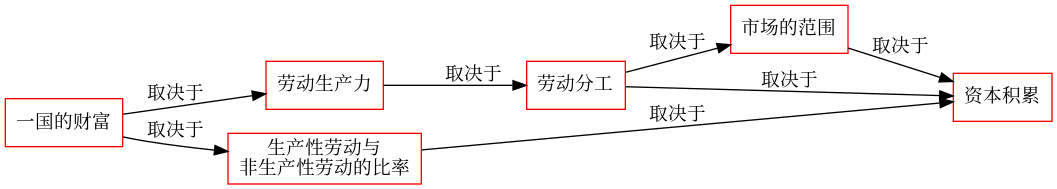
\includegraphics{simi.png}
  \caption{\label{fig:simi}一国财富的决定因素 }
\end{figure}

增加劳动力,通过机器工具或者劳动分工等提高已雇佣的劳动者的生产力,几乎都需要追加
资本。

对亚当·斯密来说,资本积累毫无疑问要求一个自由市场与私人制度框架。……在私人财产
体制中,对高资本积累率的进一步要求就是不平等的收入分配。

\section{国际贸易}

斯密主张非规制的对外贸易,理由是如果两国各自用生产成本较低的产品去交换生产成本较
高的产品,这种交换对双方来说都是有利的。用经济学的语言来说,这就是著名的对外贸易
的绝对成本学说。而且,这一学说不局限于国际贸易,它也适用于一个国家的内部贸易。

用现代经济学语言来说,随着劳动变得越来越专业化,存在收益递增(成本递减)的情形。
斯密认识到,如果两个个体出生时拥有相等的天赋并保持这一天赋不变,如果他们实行分工
并交换其产品,那么,他们中的任何一个人都不具有优势。然而,如果两个个体通过劳动专
业化变得更加熟练,那么两人所生产产品的成本都减少了,两人都从专业化与贸易中获益。
从斯密的这一见解中,产生了如下对自由贸易的发展至为关键的共识,随着时间的变化,任
何国家都能够通过专业化与劳动分工自动得获得生产某些产品的绝对成本优势,并且所有国
家都能够从此产生的国际贸易中获益。斯密认为,自由放任的政策将不断导致所有国家更高
的福利水平。

斯密在其广泛的社会科学与历史框架中,就经济分析做出的较少抽象而更多制度性的见解,
以及所使用的方法,直到今天还吸引着越来越多的注意力。政治经济学这一术语从经济学行
话中已经消失一百年了,但是,很多经济学家现在正迫切要求回归到更加斯密化的经济学范
围中,就像属于所暗示的那样。公共选择理论与新制度经济学两者的根源都能追溯到亚当·
斯密。

\section{价值理论}

价格或价格

(1)是什么决定了一件产品的价格?用现代经济学的语言来说,是什么决定了相对价格?(2)
是什么决定了价格总水平?(3)什么是福利的最佳度量标准?第一和第三个问题是现代微观
经济学的部分内容;尽管第二个问题难以用通常简单的“宏观--微观二分法”来判断,但是
一般情况下它都被包含在宏观经济学的宽广范围中。对上述任何一个问题,斯密都没有提供
明确的答案。原因在于,他自己对什么决定了相对价格的讨论,与自己试图发现不同时期福
利变化的度量相混合。
一组经济学家认为,斯密有三个相对价格理论(劳动成本、劳动支配、生产成本),以及一
个解释价格总水平的理论。另一组经济学家则认为,斯密研究了生产成本的相对价格理论,
度量不同时期福利变化的理论,以及价格总水平理论。后一组经济学家否认斯密曾涉及劳动
的相对价格理论。我们认为,斯密对这些理论都进行了试验:对于简单社会而言的由劳动成
本与劳动支配所组成的相对价格理论;对于发达经济体而言的生产成本的相对价格理论;衡
量不同时期福利变化的指数形成过程;以及解释价格总水平的理论。

\subsection{相对价格}

尽管亚当·斯密将相对价格解释为由供给或者生产成本单独决定的。但是,他并没有完全忽
视需求的作用。他认为市场价格或者短期价格是由供需双方决定的。自然价格,或者长期均
衡价格通常取决于生产成本,虽然有时斯密也表示自然价格取决于需求与供给。这些不一致
为经济理论史家们争论斯密的真正含义提供了丰富的机会。

斯密对他所处时代经济体中相对价格形成的分析,区分为两个时间段和经济体的两个宽泛的
部门,分别是短期与长期、农业与制造业。在短期或者市场阶段,斯密在制造业与农业中都
发现了向下倾斜的需求曲线与向上倾斜的供给曲线;因此,市场价格取决于需求与供给(两
个曲线的横坐标均为数量,纵坐标为价格)。斯密对长期中发生的更为复杂的“自然价
格”的分析,包含着一些矛盾。对农业部门来说,自然价格取决于供需,原因在于长期供给
曲线向上倾斜,表明成本递增。但是,对制造业部门来说,长期供给曲线有时被假定为完全
富有弹性(水平的),表明成本不变,价格完全取决于生产成本;在分析的另一些地方,又
向下倾斜,表明成本递减,自然价格就取决于供需双方。

斯密对制造业产品自然价格决定因素的陈述,存多种解释。……斯密前后一贯地注意到需求
在自然价格形成中,以及将资源在经济体不同部门之间配置时的作用。不过,无视长期供给
曲线在制造业中的形状,主要强调生产成本对自然价格的决定,这是斯密以及后来的古典经
济学家的特点。

经院哲学对相对价格问题感兴趣,原因在于他们关注交换的道德方面;重商主义者则是因为
他们认为财富是在交换过程中产生的。尽管斯密有时也从道德方面讨论相对价格,然而他对
相对价格的决定因素感兴趣还有更重要的原因。一旦经济体实行专业化与劳动分工,交换就
成为必须。第一,如果交换处于高于物物交换水平的状况下,就会存在交换媒介——货币——的
问题。第二,存在价值或相对价格的问题。用斯密的话来说就是,什么原理决定了产品的相
对价值或交换价值?第三,存在经济体的产量如何在那些参与生产的主体之间进行分割(收
入分配)的问题。

\subsection{价值的含义}

\begin{quotation}
必须注意“价值”一词有两个不同的意思。有时它表示某一特别物品的效用;有时则表示该
物品给予占有者购买其他物品的能力。前者也许可称之为“使用价值”,而后者或许可称之
为“交换价值”。那些具有最大使用价值的物品,往往几乎或完全没有交换价值;相反地,
那些具有最大交换价值的物品,却往往几乎或完全没有使用价值。没有什么东西比水更有用,
可是水却几乎买不到任何东西。相反的,钻石几乎没有使用价值;但拿钻石去交换,往往可
以得到大量的其他物品。(谢宗华《国富论》21页)
\end{quotation}

按照斯密的观点,交换价值是一种商品购买其它产品的能力——它的价格。这是市场所表达的
一种客观度量。他关于使用价值的概念是含糊的。一方面是,使用价值有道德内涵,因此是
对经院哲学的回归。比如钻石基本没有什么使用价值。另一方面,使用价值是一种商品满足
需要的能力,是因持有或消费一件产品而获得的效用——总效用、平均效用、边际效用等。斯
密的关注点是总效用,这就模糊了他对需求如何在价格决定中发挥作用的理解。(直到斯密
创作《国富论》一百年之后,边际效用与价值之间的关系才被经济学家所理解。)显然,水
的总效用超过了钻石的总效用。然而,因为商品的边际效用经常随着其消费得更多而递减,
钻石的边际效用就更高。我们愿意为一件商品所支付的价格——我们对获得又一单位商品所寄
予的价值——不仅取决于商品的总效用,而且取决于其边际效用。因为斯密对总效用的关注,
斯密就既不能为“钻石——水悖论”找到满意的解决办法,也不能了解使用价值和交换价值之
间的关系。

\subsection{斯密关于相对价格}

因为斯密对相对价格的决定因素有些困惑,所以,他发展了与这些因素相关的三个独立的理
论:(1)劳动成本价值理论;(2)劳动支配价值理论;(3)生产成本价值理论。

他假设了经济体两种截然不同的状态:初期野蛮状态或原始社会,其中资本还没有被积累起
来,土地未被使用;发达经济体,其中资本与土地不再是资源充足的产品(他们具有超过零
以上的价格)。

\begin{description}
\item[原始社会中的劳动成本理论]

按照斯密的劳动成本理论,在还不存在土地与资本的经济体中,或者土地与资本还是无限充
足的自然资源的经济体中,一件产品的交换价值或者价格,由生产产品所需的劳动量决定。
斯密认识到生产一件产品所需的劳动量不能简单地用时钟表示的时间数量来度量,原因在于,
除了时间之外,也必须考虑有关的精巧或者技能,以及任务的艰难与困苦。

在这一点上,斯密遇到了所有的劳动成本价值理论都遇到的,仍未被后来的经济学家成功地
予以解决的一个难题。如果劳动量是一个以上变量的函数,那么,我们必须找到一种方法来
说明所有变量的相对重要性。斯密试图将时间、艰难程度以及精巧程度还原为一个共同分母
的问题。

但斯密的建议仅仅是重申了问题,而不是为问题提供解决办法。其价值理论的目的是解释相
对价格的那些决定力量,但是工资本身就是其理论必须解释的经济体中的很多价格之一。斯
密利用一套价格,也就是工资,来解释另一套价格。

\item[原始社会中的劳动支配]
按照斯密的观点,在劳动支配理论中,一件产品的价值等价于产品的劳动成本。1海狸=2野
鹿。

\item[发达经济体中的劳动理论]
  资本已经被积累,土地也已被利用,它们不再是资源充足的产品。并且,一件产品的最终
  价格,也必须包括当做利润的资本家的收益以及当做地租的地主的收益。最终价格形成了
  由工资、利润、地租这些要素报酬所构成的收入。


\item[相对价格的生产成本理论]
  斯密一直努力发展经济体中产品最终价格不仅仅包含劳动成本的劳动价值理论,但是他最
  终还是放弃了下面的这种观点,即任何劳动价值理论都适用于像他所处时代一样发达的经
  济体。斯密似乎发现,一旦资本被积累起来,土地被加以利用,并且,一旦必须支付利润、
  地租、还有劳动,能唯一适当地解释价格的就是生产成本理论。在成本理论中,一件商品
  的价值取决于对所有生产要素的支付:除了劳动之外,还有土地和资本。在斯密的体系中,
  利润这一术语既包含我们今天所理解的利润,也包括利息。在斯密假设平均成本不随着产
  量增加而增加的地方,无论使用总成本还是平均成本,这一计算都能得出相同的价格。在
  斯密假设平均成本随着产量而变化的时候,价格就取决于供需双方。然而,在分析长期自
  然价格的决定时,即使当供给曲线不被假设为完全富有弹性时,斯密也强调供给与生产成
  本。斯密主张,竞争占优势的地方,商人、劳动者、地主的私利将导致与生产成本相等的
  自然价格。
\end{description}

\section{分配理论}

劳动是为大部分家庭所拥有的唯一的生产要素,因此,家庭的收入一般取决于工资率与工作
时间的长度。拥有资本的那些家庭所获得的财产收入量,取决于家庭所拥有的资本与土地的
数量以及这些要素的价格。

因为工资、利润、底足都是经济体中的价格,所以,它们的相对价格——连同个人出售的劳动、
资本、土地数量一起——决定了收入的分配。尽管收入分配不是斯密主要关注的内容,他还是
提出了几个不同的有时甚至矛盾的工资、利润、地租理论。我们将只限于涉及其分析中领先
于后来经济学家的一些方面进行阐述和批判。

\subsection{工资}

在《国富论》第一篇第八章中,他提出了最低工资理论、生产力理论、讨价还价理论、剩余
要求权理论、工资基金理论……有矛盾之处。

斯密指出,在对工资的讨价还价过程中,劳动处于劣势。他说,因为雇主比雇员的人数少,
所以雇主能够很容易地联合起来巩固他们的地位。此外,法律允许雇主联合,但是禁止雇员
组成联盟。按照斯密的说法,议会有很多反对提高工资的法案,但没有一个反对降低工资的。
最后,即使在罢工期间或停工期间不雇佣劳动,雇主也有足够的资源来维持他们的生活。但
是在另一方面,“没有工作,很多工人生存不了一星期,很少有人能生存一个月,几乎没有
人能生存一年。”在这些章节中,斯密削弱了市场力量的有益运作过程,并似乎已经意识到
其完全竞争性市场的假设收到了限制。

\subsection{工资基金学说}

斯密在对工资的讨论中,提出了他的工资基金学说,这一观点成为古典经产学的一个重要分
析工具。假定存在一个固定的资本基金,专门用以支付工资。因为生产过程是耗时的,所以
从生产过程开始到产品最终销售之间,需要以前生产的产品供劳动者用于衣食住行等。这些
库存产品或资本被称为工资基金,其来源是资本家的储蓄或者消费中断。给定劳动力和工资
基金的规模,工资率就可以确定为:工资率=工资基金/劳动力。

\subsection{利润}

令人奇怪的是,自己对利润性质与源泉的讨论极其简短。一般而言,古典经济学家都没有做
太多的努力来解释这些。显然,斯密毫无疑问地接受了下面的这种合理性,即利润是因资本
家执行了对社会有用的功能而对他的一种支付(参考工资基金等)。按照斯密的观点,劳动
者允许从其产量中进行利润的扣除,原因在于,劳动者并不拥有工作所用的原料和独立的支
持手段。于是,利润在此就由两部分构成:纯利息收入和风险收入。

在斯密的原始经济体中,劳动者获得了全部产品,但是在他自己所处的时代,劳动者不得不
与资本家和地主一起分享产品。斯密从未解释为什么要从劳动的产量中扣除利润和地租……

\subsection{地租}

斯密至少提出了四种地租理论,所有的理论都互相矛盾。地租的起源从不同角度被认为是:
(1)地主的需求;(2)垄断;(3)差异化的优势;(4)大自然的施舍。

\subsection{随着时间变化的利润率}

他对不同时期利润率的变化极其感兴趣。他预测,随着时间的推移,利润率将会下降,原因
有三。(1)劳动市场的竞争。资本积累将引起资本家之间在劳动市场上的竞争,其结果是
工资上升。斯密断言工资上升将致使利润下降。(2)商品市场的竞争。斯密推论,随着产
量增加,生产者之间的竞争加剧,结果是商品价格下降,利润减少。这也暗示了整个经济体
生产过剩的可能性,它与斯密所主张的不可能发生生产过剩的观点相冲突。(3)投资市场
的竞争。显然,斯密认为投资机会是有限的,因此,资本积累的增加将致使利润下降。当他
考察什么历史资料对研究利息率的长期趋势有用时,数据支持了他的理论推论。他的确也注
意到一些殖民地的特征是高工资与高利润并存。


\subsection{福利与价格总水平}

《国富论》第一篇第五章“论商品的真实价格与名义价格或其劳动价格与货币价格”。我们
认为,斯密试图在本章回答几个问题,尽管这些问题相互关联,但是当他们被同时加以考察
时,又会产生混淆。他努力去发现:第一,决定价格总水平的因素;第二,不同时期福利变
化的最佳度量。第二个问题更加困难。我们应当怎样用一种明确的方式来界定福利,使得福
利变化能够被度量出来呢?假设经济体制生产唯一的一种最终产品——野鹿。根据所消费的野
鹿数量,就能界定和度量经济体的福利。对社会来说,较大数量的野鹿消费代表了福利的增
加,较少数量的消费则代表福利的减少或者“不幸福”。当我们引进第二种最终产品海狸时,
问题就变得复杂了。我们能毫不含糊地说两者消费都增加,则福利也增加;两者消费都减少,
则福利也减少。但是,如果海狸的消费增加了,野鹿的消费减少了,又该怎样判断福利呢?
社会中,那些给海狸较高评价的人,他们的福利将会增加;那些给野鹿较高评价的人,他们
的福利将会减少。对于一个生产两种或者更多产品的经济体来说,有可能界定和度量其福利
的变化么?斯密试图回答这个问题。

如果用社会的总消费或者产量来界定福利,那么,对多产品的经济体来说,首先要解决的问
题就是,找到一种加总产品数量或者产品消费的方式。这一问题的一个可能的解决方案是,
将所有商品都转换为共同的度量标准。在今天的经济体中,我们通过加总每件商品的货币价
值来度量产量,已获得我们成为GDP的一个总数。从当年到下一年,如果GDP增加了,我们就
能断定福利增加了吗?

通过这种方法来度量多产品经济体中产量的变化,也呈现出一些困难。原因在于,即标准货
币本身是可变的。价格总水平变化,产量的货币价值也变化。斯密考虑了使用黄金或者记账
单位作为共同的度量标准的可能性,但又断定,因为这些商品的价格也在变化,所以在这一
用途上它们不是令人满意的。于是,他转向了劳动,但却发现劳动的价格也随时间而变化。
最后,它能够找到的用来评定福利变化的唯一不变的度量标准是劳动的负效用\footnote{负
  效用是指某种东西所具有的,不但不能给人们带来某种欲望的满足,反而给人们带来了不
  舒适或痛苦的能力。如垃圾、废气一类物品。负效用一般是在消费者消费商品得到最大满
  足程度之后出现的,因为这时消费者对该种商品消费得到的总效用已经达到了最大值,如
  果再继续增加这种商品的消费量,就必然产生负效用。}。

\begin{quotation}
所以,劳动看来显然是唯一普遍的,也是唯一精确的价值衡量标准。或者说,劳动是唯一可
让我们随时随地据以比较各种商品价值的标准。(顾版《国富论》28页)
\end{quotation}

 考虑到斯密关于能够用劳动负效用来计算福利指标的结论,度量福利变化的问题就容易解
 决了。(将货币收入与名义价格转换为实际收入与实际价格后)如果我们能用较少的劳动
 生产相同的产量,那么,我们将拥有更多的闲暇,经济状况就会更好。

 度量福利的变化远比斯密所设想的要复杂得多,然而我们不能涉及全部问题。斯密没有论
 述如何界定或度量劳动的负效用。这一点看来完全是主观的。直到20世纪,正统经济学家
 才对他的假设之一提出质疑,即较多的产品比较少的产品要好,或者说,没有增加劳动负
 效用而使产量增加,必定总会导致福利增加。在斯密的著作中,组成总产量的各种产品不
 是他关注的问题。产量的增加就是福利的改进。斯密及后来的正统经济学家,不考虑扩大
 的产量所带来的“生活质量”,他们较少注意或者不去注意以污染或其他有害外部性存在
 的成本,这些成本是为不断增大的产量所进行的预付。

 确定社会的长期增长率,是亚当·斯密主要关心的一个问题。随着我们步入21世纪,经济增
 长及其原因和结果这一问题又变得突出了。“新增长理论”,罗伯特·巴罗和阿尔伯特·F·
 阿戴斯与爱德华·L·格拉瑟等人的现代经验方法试图了解国家财富的原因。

 \section{总结}

 斯密对经济思想的贡献与影响是巨大的,大大超过他所处时代的其他任何一位经济学家。
 他领会了支配市场经济的重要观念和力量。然而他未能详细阐述关于相对价格、价格总水
 平及福利变化的单独理论,并对它们进行清楚的区分。(其他内容请看前文,不再摘抄)。

 斯密并不是一个纯粹的理论家。相反,他是一位政治经济学家,他能够用描述性的和历史
 的材料来补充市场经济中不同部门相关性这一极其重要的认识……穆勒追随纯粹的理论家
 李嘉图,马歇尔又追随穆勒;穆勒与马歇尔都试图使经济学回归到亚当·斯密前后关联的分
 析与政策上来。很少有例外的是,马歇尔以来的正统经济学家的分析方法,几乎专门集中
 于纯粹的抽象理论,很少关注历史与制度材料,抛弃了斯密的方法论。然而,抛弃了斯密
 自由放任政策主张的非正统经济学家却一直延续着他的方法论。

 \chapter{李嘉图与马尔萨斯}

 李嘉图是金融世界的人士,马尔萨斯则是精神世界的人物。

 \section{大卫·李嘉图——一个理论家的理论家}

李嘉图是一个由股票经纪人转变而成的经济学家,他对经济理论的许多领域都作出了重要贡
献,包括方法论、价值理论、国际贸易、公共财政、收益递减、地租。

\subsection{斯密《国富论》与李嘉图《原理》之间的时期}

李嘉图《政治经济学及赋税原理》1817年出版之前,亚当·斯密1776年出版的《国富论》一
直支配着英国的思想。这期间的四十年,尽管对经济分析有一些重要贡献,但是未出现过重
要的经济理论。托马斯·罗伯特·马尔萨斯在1798年发表了一篇短文,1803年出版了一部著作,
都是关于人口的;1815年,韦斯特、托伦斯、马尔萨斯及李嘉图分别发表了地租概念和经济
意义的短文。

因为马尔萨斯的人口论题对于理解李嘉图理论的某些部分是基本性的,所以我们将首先考察
它;然后再讨论和评价李嘉图;最后,又将回到马尔萨斯,考察他在,政治经济学原理》
1820中所发展的关注经济体在充分就业下自动运转能力的观点。作为经济思想发展中最生动
的辩论之一,马尔萨斯与李嘉图激烈地辩论过这一问题。

\section{马尔萨斯的人口学说}

马尔萨斯的主要论题是人口增加快于食物供给增加,这一观点并不是由他最早提出的。斯密
与本杰明·富兰克林等人的著作中也能找到这一论题。然而马尔萨斯对人口问题的论述影响
最大。

\subsection{对时代问题进行思考性回应的人口理论}

似乎有三个因素。第一个因素是人口对食物供给造成的压力。1790年后,英国进口食物成为
必需,价格也显著上升。第二个因素是低收入阶级在工厂生产代替家庭生产、英国开始城市
化背景下的日益贫困。第三个因素是发生在罗伯特·马尔萨斯与其父丹尼尔·马尔萨斯之间的
争论。丹尼尔·马尔萨斯所接受的戈徳温和康德桑特的基本观点是:个人的特性并不是通过遗
传而获得的,而是通过他或她生活的环境塑造的。戈徳温尤其为他所赶到的周围世界的艰难、
贫困、不幸以及恶行所困扰。他断言,对此负主要责任的是政府,也因此被一些人称为哲学
无政府主义之父。罗伯特·马尔萨斯尤其试图证明,贫穷与不幸并不是社会制度与政治制度的
结果,这些制度的变革不会消除社会的罪恶。罗伯特·马尔萨斯于1798年匿名出版人口论,书
籍全名为“影响社会将来改善的人口原理论说,并评戈德温等学者的学说”

\subsection{人口论题}

马尔萨斯在其短文第一版中所确立的基本原理,建立在两个假设之上:(1)食物对于人类
的生存是必须的,(2)两性之间的性爱是必须的并将保持不变。他推断,与食物供给相比,
人口趋向于以更快的速度增长,这就是贫穷与不幸的原因。尽管马尔萨斯承认土地供给的有
限性,但是他没有利用农业中的收益递减原理来证明经济体不能显著地增加食物供给这一主
张是正确的。……马尔萨斯不认可技术的发展有可能解决人口问题,这也使他的很多理论无
效。

他断定人口控制将会逐步使人口增长率符合食物供给增长率。第一版中,他假定了积极的与
预防性的这两种类型的人口控制。积极的人口控制即通过战争、饥荒、疾病以及类似的灾难
来提高死亡率。预防性的人口控制即降低出生率,它功过延缓婚姻而得以实现,但他也认为
晚婚不可避免会产生婚前性行为,从而仍然会产生苦难、堕落等社会问题。

\subsection{关于人口论题的争论}

1803年,马尔萨斯发表《人口论》第二版,与第一版有差异。他不再试图批评他的父亲、戈
徳温以及康德桑特的观点。取而代之,他决定用一种现有数据所许可的科学方式来清晰说明
人口问题。第一版方法完全是演绎的,他在第二版中稍微进行了归纳,并通过统计数据来支
持论点。

在第一版中,人口不受控制导致恶行与不幸。第二版中引进了一种新的人口控制:道德限制,
或者说,无力赡养子女的人不要结婚,并且在婚前要保持贞操。这种新的控制,摧毁了马尔
萨斯反对乌托邦的部分主张,但是他不再关注于反驳乌托邦。

\begin{description}
\item[马尔萨斯的人口论题] 他从来不严肃地讨论通过避孕的方法控制人口的可行性。此外,
  马尔萨斯对为了有孩子而发生性关系的本能欲望感到困惑。尽管在所有社会的人群中,性
  冲动都是强烈的,但是日益提高的富裕程度和教育水平,趋向于在性欲与生孩子决策之间
  产生差别。另一个难点是马尔萨斯的武断假设,即食物供给的增加无法快于人口的增加。

  马尔萨斯的人口论题在古典经济学的理论与政策中找到了应用。由斯密提出,李嘉图及其
  追随者予以扩展的工资基金学说,意味着劳动的实际工资提高将导致人口增加,并最终使
  工资率恢复到以前的水平。因此便存在下面的争论,即提高社会上低收入群体经济福利的
  任何尝试,都将受挫于人口规模的增加。……古典经济学家利用马尔萨斯人口学说作为反
  对穷人法的论据。他们通过结合马尔萨斯论题与工资基金学说而完成的对工资率的分析,
  被称为工资铁律(the iron lay of wages)。

  英国自然学家查尔斯·达尔文和A.R·华莱士各自阐明了众所周知的达尔文进化论。两人都
  承认,马尔萨斯对他们的思想产生了重要影响。

  大卫·李嘉图将马尔萨斯的人口理论组合到古典政治经济学中。
\end{description}

\section{李嘉图:方法、政策、范围}

李嘉图对经济思想发展的影响超过了他对纯经济理论的贡献,也使经济学家偏离亚当·斯密
所提倡的经济学方法与范围,改变了研究方向。

\subsection{李嘉图的方法}

斯密用两种方式来处理政治经济学问题:(1)运用演绎理论来分析他所处时代的经济体;
(2)呈现同时代人描述性的、非正式的叙述以及呈现历史上的制度。斯密的方法将理论与
历史上的描述性材料相混合。在另一方面,李嘉图代表了忙碌的纯理论家。他从他所处时代
的经济体中进行抽象,构建了基于演绎方法的一种分析。他的技艺如此杰出,以至于今天他
还为纯理论家们所钦佩,即使他的数学技能略显笨拙。但是,李嘉图的经济学具有强烈的政
策导向。他所处时代亟待解决的问题是对进口到英国的谷物征收关税以及关税对收入分配的
影响。

\subsection{李嘉图与经济政策}

李嘉图关注当时英国升高的谷物价格、地租以及英国经济结构变革所导致的更为普遍却极端
重要的问题——工业的相对增长与农业的相对下降。……问题集中于实行自由的国际贸易还是
规制的国际贸易。

李嘉图的政策方法对后来经济学家政策制定方式的发展具有重要影响。他对一项好政策的表
达方式是从非本质的事物中进行抽象,构建一个揭示变量之间因果关系的高度理性化的模型。
当理论模型用来制定经济政策的基础时,为了获得较强的理论结论,有必要抽象掉甚至冻结
一些可能对结果有重要影响的变量。李嘉图这种非关联的理论化政策制定方式,其难点在于:
在现实世界的政策制定中,这些“被冻结”的既定变量经常是开放的,并会产生意想不到的
结果。李嘉图的方法(高度抽象)与他的政策方法(非关联)最终成为主流经济思想所奉行
的道路。

李嘉图主义的两个成分一直保留到今天:高度抽象的理论和基于抽象模型的非关联的政策制
定,前者通过假设消除了如此多的变量,以至于最终的结论没有争论的余地。

\subsection{李嘉图思想所界定的经济学范围}

在经济学的基本任务这一观念上,李嘉图代表了一个转折点。亚当·斯密延续了重商主义对
国民财富决定力量的关注。李嘉图则主张经济学的主要目的是确定支配地主、资本家以及劳
动者之间收入分配的法则。

李嘉图全神贯注于现在被称作收入的功能性分配的研究,收入的功能性分配是指年产量流向
劳动、土地及资本的相对份额。在现代国民收入账户中,国民收入被界定为按照要素价格对
生产要素进行的支配。当现代理论家分析收入的功能性分配时,他们经常使用经济体的总生
产函数这一概念。

李嘉图尤其被不同时期收入的功能性分配的变化所吸引,在他的体系中,这是宏观经济学的
一部分。他在由三个阶级组成的社会背景下考虑这一问题:获得利润与利息的资本家、获得
地租的地主以及获得工资的劳动者。像斯密一样,李嘉图不得不在微观层面上阐明理论(尽
管李嘉图的确考虑了许多其他宏观问题,例如人口理论、工资基金学说、劳动力规模、价格
总水平以及经济体的短期和长期稳定)。他特别对导致不同时期收入变化的因素感兴趣。然
而,他主要关注收入分配变化对资本积累率与经济增长率的影响。因此,他的工作具有如下
效果,即把后来的经济研究引导到微观经济问题而不是宏观经济问题上,这一效果与他的意
图恰好相反。

\section{李嘉图的模型}

在经济活动中,资本家充当了主要角色:他们是生产者、指挥者以及最重要的参与者。他们
为经济体执行两个主要功能。第一,他们有助于资源的有效配置,原因在于他们将资本转移
到收益最高的领域,在这一领域中,如果完全竞争性的市场占优势,那么消费者需求就能以
最低的、可能的社会成本得到满足。第二,他们通过储蓄与投资来发动经济增长。

尽管李嘉图采用劳动成本理论来解释不同时期相对价格的变化,但在他的模型中,劳动在本
质上是被动的。他使用工资基金学说与马尔萨斯的人口理论来解释劳动者的实际工资:实际
工资=工资基金/劳动力。工资基金取决于资本积累,劳动力规模受马尔萨斯人口理论的支配。
如果作为资本积累的结果,工资基金、短期实际工资、人口、劳动力将以此增加。当劳动力
充分增加,使实际工资恢复到与文化相关的维持生活的最低水平时,便存在长期均衡。

显然,对什么是维持生活的看法,随着时间和文化的不同而不同。李嘉图所说的维持最低生
活水平的工资,并不是一个客观的不变的福利水平,而是与特定时间与文化相联系的。

在李嘉图的体系中,地主仅仅是寄生虫。在李嘉图看来,土地的供给曲线是完全无弹性的,
土地的社会机会成本为零。地主获得地租收入,仅仅是因为拥有一种生产要素,他并没有提
供任何对社会有益的作用。

李嘉图模型中,$总收益 - (维持最低生活水平的工资+折旧)=净收益$。因此,经收益由利
润、地租以及维持最低生活水平的工资之上的部分组成。在长期均衡中,工资将处在维持最
低生活水平的工资上,净收益就等于利润加上地租。工人与地主总是将他们的全部收入花在
消费商,因此利润成了储蓄或资本积累的唯一来源。李嘉图断定,作为经济增长率减小的结
果,当利润下降、地租上升时,随着时间的变化,将会发生有利于地主的收入再分配。

\subsection{时代难题:《谷物法》}

关于这一时期谷物法,引发广泛争议。很多主张扰乱了李嘉图。其中之一是较高的关税将导
致较低的谷物价格。这种主张认为,较高的关税鼓励英国农业中更多的投资,结果是产量或
供给增加,当他们进入市场时谷物价格将会下降。李嘉图不同意这些结论。另一个主张是谷
物的高价格是高地租的结果。按照这一推理,地租是决定价格的因素。李嘉图也不赞同,他
辩论说地租是价格被决定的因素。李嘉图清楚认识到谷物法的根本问题在于收入的分配。较
高的关税将使收入有利于地主。

\subsection{分析工具与假设}

当李嘉图试图处理由《谷物法》争议所引起的很多政策问题时,他利用了很多分析工具与假
设,发展出一个精细的扩展模型。在考察其理论之前我们应当先熟悉这些工具和假设。

\begin{enumerate}
\item 劳动成本理论:不同时期相对价格的变化,可用以时间度量的劳动成本的变化来解释。

\item 中性货币(neutral money):货币供给的变化,可以引起绝对价格与相对价格水平
  两者的变化。然而,与货币供给变化所引起的其他现象不同,李嘉图对不同时期相对价格
  的变化更感兴趣,所以他在其模型中假设,货币供给的变化不引起相对价格的变化。

\item 劳动与资本的固定生产系数:只能使用劳动与资本投入的一种联合来生产既定的产量。
  对每种类型的经济生产而言,技术上的考虑使得劳动——资本比例是固定的,且不随着产量
  的变化而变化。


\item 制造业收益不变,农业收益递减:制造业的供给曲线是水平的,或者完全富有弹性的。
  农业供给曲线向上倾斜(随着产量扩张,边际成本递增)。


\item 充分就业:长期中,经济体在资源充分利用的水平上趋向自动运转。


\item 完全竞争:市场包含很多独立的生产者,他们的产品具有同质性,任何一个单独的销
  售者都不能影响市场价格。


\item 经济参与者:个人在他们的经济活动中都是理性的和精于计算的。资本家为获得最高
  的利润率,工人为获得最高的工资,地主为获得最高的地租而努力。在完全竞争性市场中,
  这样一种社会的相互作用,将导致具有类似风险的投资,其利润率统一,具有相同技能与
  培训的劳动力,其工资水平统一,具有相同肥力的土地,其地租水平相同。

\item 马尔萨斯人口论:人口趋向于以快于食物供给的速度增加。

\item  工资基金学说:工资率等于工资基金除以劳动力规模。
\end{enumerate}

\section{李嘉图的地租理论}

\subsection{收益递减}

\subsection{从产品一方看地租}

李嘉图主张,之所以存在地租,是基于如下原因:(1)肥沃土地的稀缺性;(2)收益递减
规律。

李嘉图将地租视为给地主的一种支付,它等于不同肥力土地上的利润率。在竞争性市场上,
市场力量的运行使两种级别土地的利润率相等。

假设A级土地使用3个单位的劳动与资本组合,B级土地使用2个单位的组合,C级使用一个。如
图所示。集约边际描述了追加资本与劳动组合对既定地块的影响,反映了边际收益递减原理。
如果地租是对地主的支付,它等于不同级别土地上的利润率,那么A级土地地租
为 $270-80\times 3 = 30$ ,B级地租为 $170- 80 \times 2 = 10$ ,C没有地租。

\begin{table}[htbp]
  \centering
  \caption{集约边际与粗放边际(用蒲式耳计算的边际产品)}
  \label{tab:lijiatu}
    \begin{tabular}{@{}c  c c c@{}}
      \toprule
      \multirow{2}*{} & \multicolumn{3}{c}{\shortstack{粗放边际 \\ \tikz [ultra thick] \draw [->] (0,0) -- (2,0);}} \\ \cline{2-4}
      &地块A & 地块B & 地块C  \\ \midrule
      \multirow{3}*{\tikz [ultra thick] \draw [->] (0,1) -- node[left]{\shortstack{集\\约\\边\\际}}(0,0);} & 100 & 90 & 80  \\
      & 90 & 80 & \\
      & 80 & & \\ \bottomrule
    \end{tabular}%
\end{table}

\subsection{从成本一方看地租}

随着连续投入劳动与资本组合,A级土地的边际产品下降。表述这一结果的另一种方式是说,
随着土地更加集约化耕作,生产谷物的边际成本上升。边际成本被界定为生产最终产品的一
个增加量所需增加的总成本。假定资本与劳动的一单位组合在市场上卖100美元,在A级土地
上生产第100蒲式耳谷物的边际成本就等于1美元,第190蒲式耳谷物的边际成本为1.11美元
($100/90$),最后一单位蒲式耳谷物的边际成本为1.25美元($100/80$)。B级、C级土地
上生产的最后一单位蒲式耳谷物的边际成本也等于1.25美元。如果完全竞争性市场存在,一
定是这种情形。在长期均衡小,根据定义,当三种级别土地上的边际实物产品相等时,增加
量的边际成本必定相等。

从成本一方来度量地租,不是使用小麦的蒲式耳数,而是使用货币。销售者之间的竞争使得
市场上只有一个价格,该价格等于最低效率下生产出来的谷物的边际成本。在竞争性市场中,
个别厂商的供给曲线就是他们的边际成本曲线,行业供给曲线是个别厂商供给曲线的加总。
因假设一单位劳动与资本的总成本是100美元,那么对A级土地来说,总收益是$270 \times
1.25 = 337.5$美元,地租为37.5美元。B级土地地租为12.5美元。

这一简单的农业模型揭示出地租概念和竞争性市场运作的几个要点:(1)市场中农场主之
间的竞争,将促使谷物价格等于成本最高的单位产量的边际成本;(2)对土地的竞争,将
使得地租支付给拥有最肥沃土地的地主;(3)竞争将导致所有级别土地具有统一的利润率。
甚至在今天复杂的经济体中,这些相同的竞争性力量都对价格、地租以及利润的决定有影响。
因此在李嘉图的方案中,地租是价格被决定的因素,而不是决定价格的因素。谷物的高价格
不是由高地租决定的;高地租是由高的谷物价格决定的。

能够看到,《谷物法》所施加的进口限制,使得集约边际与粗放边际向下推进,其原因在于
肥沃土地的稀缺性和收益递减原则。新增劳动与资本组合的边际实物产品将下降,这就等于
说边际成本将上升,其结果是谷物价格与地租都上升了。

在李嘉图对地租的分析中,他声称地主的地租性收入是一种不劳而获的收入,这非常适合对
地租征税。1879年,美国人亨利·乔治的《进步与贫困》极大地推动了对土地征税这一观念。
乔治提倡对土地征收一种能完全消除地租的税。他主张,如果所有的土地都如此征税,所产
生的收入将足以支付政府的所有支出。单一税运动。

\subsection{对地租概念更一般的看法}

今天,大部分经济学家都同意李嘉图的如下观点,即将社会作为一个整体来看,地租并不是
生产成本,因此,也不是价格的决定因素。土地的数量接近固定;因此,当供给的数量不增
加时,需求的增加将导致较高的价格(地租)。从这个角度来考虑地租,土地的机会成本为
零。

然而,从社会个别成员的角度来看,地租就是生产成本,从而是价格的决定因素。想要在生
产过程中使用土地的人,或者想要利用土地价值的人,面临他人竞争,必须为获得并保留土
地的服务进行支付。如农场主的地租数量等于土地的机会成本——等于土地在可替代的其他用
途上能够获得的地租数量。

\subsection{李嘉图的价值理论}

马尔萨斯主张对进口谷物提高关税将有益于英国,李嘉图则赞同国际贸易,反对关税。

李嘉图与贸易保护论者都同意较高的关税将导致较高的货币工资。双方都赞同,随着不太肥
沃的土地被加以利用以及耕种的土地得到更多的精耕细作,关税的提高将使土地边际量向下
推进,结果是谷物的生产成本增加。为了使工人维持最低生活水平,就要提高货币工资(工
人食物预算)。利用斯密的价值理论,贸易保护者认为较高的货币工资不一定减少利润。

一些贸易保护论者也提出,取消或降低谷物关税,将使食物价格与货币工资下降,最终引起
所有价格的普遍下降,从而导致经济衰退。因此,为了确定取消谷物关税对英国带来的利益,
李嘉图试图反驳当时盛行的生产成本理论。

大多数价值理论者试图解释既定时间点上相对价格的决定力量。然而,按照李嘉图的观点,
价值理论的主要难题是解释导致不同时期相对价格变化的经济力量。利用不变价值的度量,
我们就能够确定,如果海狸价格上升,那么它是因为海狸生产变得更加昂贵,还是因为野鹿
生产变得不太昂贵。

李嘉图花费了一些精力试图阐明不随时间而改变的绝对价值的度量。但是,李嘉图还是没能
令人满意地阐明绝对价值的度量。因此我们转向李嘉图对价值的主要关注点:是什么导致了
不同时期相对价格的变化。

\subsection{李嘉图的劳动成本价值理论}

李嘉图与斯密的价值观点不同。他在《原理》开头写道:“商品的价值或它所能交换的任何
其他商品的数量,取决于商品生产所必须的相对劳动量,而不取决于支付这一劳动的报酬的
多少。”李嘉图想强调斯密在阐明相对价格的劳动成本理论时,受到混乱与循环推论的限制,
李嘉图自己则没有为此干扰。通过下面的论断,即支付给劳动者的工资是对必要劳动时间的
度量,斯密已经解决了生产一件商品所必须的劳动量的度量问题(技能、难易程度、精巧问
题)。李嘉图认为,这是一个循环推论,在他的开篇语中,他明确地表示,价值取决于生产
所必须的劳动量,而不取决于支付给劳动者的工资。

斯密在“钻石--水悖论”中阐述过使用价值与交换价值的混淆问题,但他没有看到使用价值
与交换价值之间的联系。与斯密不同,李嘉图主张,使用价值尽管不是交换价值的度量,但
是,对交换价值的存在来说却是基本的。用现代术语来说,李嘉图是在说,商品在市场上具
有实际价格之前,必须存在一种需求,但是需求并不是对价格的度量。能够产生效用的商品
的价格具有两种来源:它们的稀缺性及生产他们所需的劳动量。

名贵的绘画、古币、酒等,他们的供给不能增加,供给曲线完全没有弹性。李嘉图说“他们
的价值与最初生产时所需的劳动量完全无关,而是随着那些愿意拥有它们的人的财富和偏好
的变化而变化。”

竞争性生产所生产的产品

李嘉图将那些稀缺的、不能自由地再生产的商品从他的劳动价值理论中排除出去,原因在于
他们“只占市场日常交换商品中的很小部分”。因此,他的价值理论只适用于能够自由地再
生产的商品以及完全竞争性市场所生产的商品。他假设经济体中制造业部门所生产的产品的
供给曲线完全富有弹性,这就是说对于制造业而言,他假设成本不变。对于农业部门,李嘉
图假设成本增加,所以,供给曲线向右上方倾斜。

分析完斯密对相对价格决定因素的解释之后,李嘉图放弃了劳动支配理论与生产成本价值理
论,而赞成劳动成本价值理论。尽管亚当·斯密否定了资本与劳动获得收益的经济体中的劳
动成本理论,李嘉图却主张,这一理论对于他自己所处的时代来说是适合的。

\begin{quotation}
  亚当·斯密,看到了在生产中,劳动者的工资同他的生产物价值不相等,看到了当作资本,一个
  商品的价值增殖,不是比例于它里面的劳动,而是比例于它支配的别人的劳动。因此,他就主
  张。在资本主义开始以后,商品的价值就不再是由生产它所必要的劳动来决定,而是由它所
  能购得的或支配的活劳动来决定。

  李嘉图正确地指责了亚当·斯密的这种混乱,说明生产商品所消耗的劳动量,和这一商品所能
  支配的活劳动量或劳动报酬是不相等的。商品中包含有多少劳动,和这种劳动有多少归劳动
  者自己是没有关系的,后者的变动并不影响前者;并且,既然承认商品中所含的劳动,在工资
  成立以前,已经是价值的尺度,就没有理由再说,在工资成立之后,它就不再是价值的尺度了。
  但李嘉图是没有真正认清亚当·斯密的错误所在的,因此,他的这种指责,也就不可能击中要
  害,将问题予以解决。

  亚当·斯密的错误,在于他混同了劳动量与劳动价值,没有能够把劳动价值与劳动力的价值
  区别开来。他不了解劳动的价值仅仅是劳动力价值的转化形态。因此,他就提出了劳动量
  决定商品价值与劳动价值决定商品价值的双重观点。其实其劳动价值决定商品价值的观点,
  是一种错误的循环论证。(《李嘉图著作和通信集(一),中译本序言)
\end{quotation}

\subsection{劳动成本价值理论的难点}

我们下一步的任务是简要说明李嘉图对五个基本问题的解决,这些问题是任何准备发展劳动
价值论的理论家都要面临的:(1)度量劳动量;(2)反应劳动技能变化这一事实;(3)
将资本产品当作影响价格的因素来加以说明;(4)在价格决定中说明土地;(5)在价格决
定中说明利润。

\begin{description}
\item[劳动量的度量] 斯密不愿意使用钟点或者实践作为劳动量的度量,因为他认为劳动技
  能与工作的艰难也是相关的。他主张,对技能与艰难的评估,通过市场中的“讨价还价与
  商谈”得以确定……李嘉图看出,斯密的逻辑是错误的,恰恰是劳动量决定了相对价格,
  而不是支付给劳动者的工资。李嘉图的解决办法是,通过用生产一件产品相关的时间量来
  度量劳动量,即只通过时钟的钟点来度量。


\item[劳动的不同技能] 熟练劳动问题。劳动不是同质产品,所以一小时的劳动的时间,可
  能生产出不同的产量。李嘉图仍用支付给劳动者的工资来度量他们的相对生产力,来解决
  劳动技能问题。从表面上看,李嘉图使自己陷入了斯密一样的循环推论,因为相对工资就
  是价格,它却被用来解释相对价格。可使,李嘉图的推论并不是循环推论,原因在于,他
  没有试图解释某一时点上的相对价格,而是设计了一种理论来解释不同时期相对价格的变
  化。

  他在回应循环推论的异议时指出,因不同技能而产生的支付给劳动者的工资差别,如果在
  不同时期保持不变,那么,最终产品价格的变化,将不是由支付给劳动者的工资引起
  的。……李嘉图关于支付给拥有不同技能劳动者的工资,在不同时期保持不变的假设存在
  有问题的地方;但是,如果承认这一假设,并考虑到他所试图解决的问题,他用时钟的钟
  点来度量劳动的办法就不是循环推论。


\item[资本产品] 几乎所有商品的生产都要求使用劳动与资本两种因素。在劳动成本理论中,
  资本对最终产品价格的影响是怎样的呢?李嘉图通过如下办法来处理这一问题,即把资本
  当成是储藏起来的劳动,也就是在以前阶段被使用的劳动(过去劳动)。劳动与资本共同
  生产的商品,其所包含的劳动量,由立刻被使用的劳动量,加上储藏在用来生产最终产品
  的资本产品中的劳动量来度量。(资本产品中有一些消耗和贬值)那么,使用这一资本产
  品生产一件最终产品所需的总劳动,就等于立刻使用的劳动小时数,加上资本产品消耗的
  一小时劳动。

  李嘉图对资本产品问题的解决,并不完全令人满意,李嘉图加总过去所有的劳动与利息成
  本,这与专门基于劳动的价值理论不一致。


\item[地租] 一旦土地成为一种经济产品,亚当·斯密的劳动价值理论就无法得到发展,这
  也是他转向生产成本理论的一个原因。李嘉图通过其地租理论解决了这个问题。在他看来,
  一蒲式耳小麦的价格取决于最低效率下生产的蒲式耳小麦的边际成本。价格是在边际量下
  被确定下来的,边际量上没有地租。正像我们看到的那样,地租是被价格决定的,不
  是决定价格的因素。因此,不同肥力土地所获得的地租,不会影响不同时期相对价格的变
  化。


\item[利润] 任何劳动价值理论所固有的另一个难点是确定利润的角色。如果利润是不同商
  品最终结果的一个不同百分比,那么相对价格或者相对价格的变化,就不能单独通过劳动
  而被准确地加以度量。劳动密集型和资本密集型、资本周转速度的不同(固定资本与流动
  资本之间的比例)都有不同利润。

  李嘉图推断,这些问题不会改变他的基本主张,即不同时期相对价格的变化,取决于包含
  在商品中的相对劳动量的变化。他的结论是,利润率的影响在数量上并不重要。
\end{description}

\subsection{李嘉图主张劳动价值理论吗}

这个问题从两个方面困扰着经济思想史学家:(1)李嘉图主张劳动价值论吗?(2)李嘉图
改变了他对劳动价值论有点的看法吗?李嘉图并不主张理论上的劳动价值理论,原因在于,
他承认生产产品所要求的劳动量的变化,并不是导致相对价格变化的唯一力量。然而,他的
确认为,解释相对价格的变化时,生产产品所必须的劳动量的变化,在数量上是最关键的成
份。

乔治·斯蒂格勒(1911-1991)在对李嘉图的理论进行分类时,将93\%归为劳动价值理论。

\subsection{李嘉图价值理论总结}

(1)与亚当·斯密相反,李嘉图主张,使用价值对交换价值的存在来说是有必要的。(2)
仅仅对于那些在纯粹竞争的市场条件下生产的、能够自由地在生产的产品来说,他的劳动价
值理论才得到发展。(3)他的主要关注点是,解释导致不同时期相对价格变化的经济力量。
(4)尽管市场价格或者说短期价格的变化,可能由很多需求与供给因素所决定,然而自然
价格或者说长期均衡价格的变化,却通过生产商品所要求的劳动量的变化得到解释。(5)
尽管某些因素修改了这些原理,尤其是利润这一因素,但是,它们没有扰乱如下本质结论,
即价值理论中,相对价格的变化多半是用生产产品所需的劳动量来解释的。

\section{李嘉图的分配理论}

李嘉图主要关注的三个问题:在某一时点上,什么决定了收入在工资、利润以及地租之间的
功能性分配;随着时间的发展,不同时期的收入分配将会怎样;《谷物法》给收入分配与经
济增长速度造成的后果是什么。在李嘉图发展价值理论与地租理论之前,他未能回答这些问
题。

\subsection{分配理论}

借助简单的曲线图,我们能从李嘉图的模型中,逐步看到他关于分配的主张。在模型中,资
本与劳动的组合以固定的比例被添加到经济体可利用的数量固定的土地上。

\begin{figure}[ht]
  \centering
  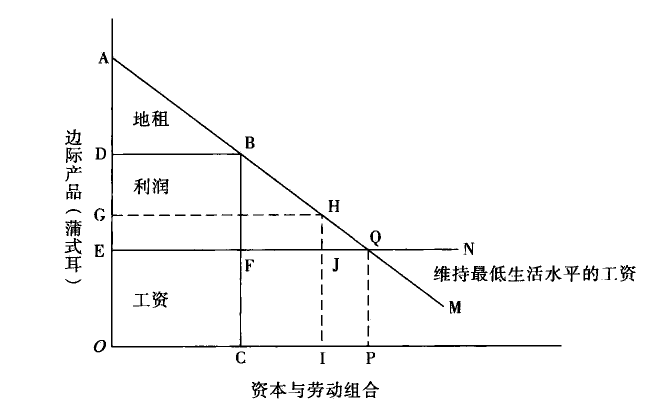
\includegraphics[scale=0.8]{lijiatu.png}
  \caption{\label{fig:lijiatu}静止状态 }
\end{figure}

曲线ABHQM代表了这些边际实物产品。假设距离OC所表示的资本与劳动组合以某一数量投入
到可利用的土地上……所投入的最后一单位资本与劳动组合的边际产品由距离BC表示,模型
中总的农业产量等于面积OABC。李嘉图的问题是确定总产量在工资、利润、地租之间的分配。
李嘉图的分析是灵巧的,因为有三个变量要确定,他通过减法来获得不同份额。正因为这一
原因,李嘉图的收入分配理论经常被称为剩余理论。

维持最低生活水平的工资,通过马尔萨斯人口理论得出,在我们的例子中,假定工资是直
线EFJQN。于是工资率就是FC,总工资是面积OEFC。……需要注意到,利润水平取决于最后
一单位资本与劳动组合的边际产品及维持最低生活水平的实际工资。

\subsection{不同时期的收入分配}

斯密预测,作为劳动、投资以及商品市场竞争的结果,随着时间的推移,利润率将下降。李
嘉图赞成这个观点,但他否认了斯密的所有理由。

斯密的第一个理由与他自己的生产成本价值理论不一致。随着劳动市场竞争加剧和工资上升,
在生产成本价值理论下,没有理由断定利润必定下降。李嘉图通过运用马尔萨斯的人口学说
来反驳斯密,他指出,如果竞争的确抬高了实际工资,那么,人口的增加将在长期中扩大劳
动力的规模,于是工资又将下降到以前的水平。

他通过萨伊定律的主张来反驳斯密关于下降的利润、投资市场与商品市场上竞争的第二个和
第三个理由。李嘉图认为,斯密对利润下降的第二个和第三个解释意味着存在普遍的产出过
剩。其原因在于投资市场的竞争只有在下列条件下才导致利润下降,既不可能按照以前的价
格销售由于新的投资而增加的产量。李嘉图认为,由于新的投资而增加的产量,能够按照以
前的价格销售掉;因此,利润率不会下降。他用同样的主张来反驳斯密关于利润下降的第三
个理由,指出商品市场的竞争不会导致价格总水平下降。在本章末尾,我们将再次考虑萨伊
定律。

李嘉图认为利润将下降,但理由是:早期经济体以高利润和高资本积累率为特征,原因在于
资本积累的源泉是利润。这种资本积累提高了利润率,结果实际工资上升,依照马尔萨斯人
口学说,人口规模将增加。增加的人口要求大量的农业产品……级差地租,地租上升与利润
下降,直至利润率接近为零、资本积累停止。

随着农业利润率的下降,资本将转移,以利用制造业较高的利润率。然而,长期均衡下,整
个经济体中各处的利润率都相等;所以,随着农业中利润率的下降,制造业中的利润率也必
将下降……最终达到所谓的古典静止状态。

利用上图,随着成长的经济体中资本积累与人口增长的发生……如果边际量得到扩展,使OI
表示所投入的最后一单位资本与劳动组合,那么我们会发现,新的更高的地租水平是面积
GAH;利润减少为面积EGHJ;总工资现在是OEJI。随着边际量被推出更远,地租水平提高,
知道总产品只由工资与地租组成、利润等于零为止。这就是静止状态;当OP这么多资本与劳
动的组合被运用时,就达到了这一状态:地租为EAQ,工资为OEQP,利润为零。

\subsection{回到《谷物法》}

尽管李嘉图已经断定,经济体的长期趋势将会导致收入的重新分配,即从资本家流向地主,
然而他之所以反对《谷物法》,是因为它加速了这一过程。因为经济增长的源泉是资本家的
资本积累,所以《谷物法》减缓经济增长速度、加快静止状态到来这一不受欢迎的后果。

李嘉图还提出了第二个主张来反对《谷物法》,即对国际贸易的阻碍减少了世界上所有经济
体的福利。为了了解这一推论,我们必须先来考察他的比较优势学说。

\section{比较优势}

应用于国际贸易中的比较优势学说,明显地体现了李嘉图头脑的极端精明。亚当·斯密对产
品跨国界的自由运动所获得的收益进行了分析。李嘉图拓展了斯密的分析,强调了自由贸易
主张。

用国际贸易理论的术语来说,如果一国在一种商品的生产中拥有绝对优势,另一国在另一种
商品的生产中拥有绝对优势,那么通过专门生产那些生产成本最低的商品,各国都能获益。

\subsection{绝对优势}

通过每单位劳动成本来衡量一国相比它国是否有绝对优势。

\subsection{比较优势}

但是,当一国在所有商品的生产上都更有效率时,又会怎样呢?

% Please add the following required packages to your document preamble:
% \usepackage{booktabs}
% \usepackage{graphicx}
\begin{table}[htbp]
  \centering
  \caption{每单位劳动的产量}
  \label{tab:bijiaoyoushi}
    \begin{tabular}{@{}ccc@{}}
      \toprule
      \textbf{国家} & \textbf{酒(加仑)} & \textbf{布(码)}   \\ \midrule
      英国 & 12 & 6   \\
      葡萄牙& 8 &  1  \\ \bottomrule
    \end{tabular}%
\end{table}

与葡萄牙相比,英国在两个行业都具有绝对优势,两种产品用劳动时间度量的生产成本在英
国都较少。然而,决定国际贸易是否有益的关键因素是比较优势,而不是绝对优势。比较优
势是通过考察每个经济体内部的相对生产力来予以确定的。

在这个例子中,英国在布匹生产上具有比较优势。即在英国,每码布匹新增产量意味着两加
仑酒的损失,而在葡萄牙,为了多获得一码布必须放弃8加仑的酒。葡萄牙在酒生产上具有
比较优势。即在葡萄牙,只用1/8码布的损失,就能多获得一加仑的酒,而英国必须放弃1/2
的布,才能生产出一加仑的酒。

在7.9加仑酒交换1码布与2.1加仑酒交换1码布的价格之间,英国与葡萄牙两个都能从交易中
获益。

依靠比较优势学说,李嘉图证明了,国际贸易收益的决定因素不是绝对优势,而是相对优势。
尽管英国在每个行业都拥有绝对优势,但只要葡萄牙在一个行业拥有比较优势,英国就能从
与葡萄牙的贸易中获益。

在李嘉图关于资源充分利用的假设下,如果要生产更多的任何一种产品,随着资源从收缩性
行业向扩展性行业转义,一些产品的产量必须被减少,多生产的产品的成本,将通过所损失
的产品数量得到度量。

\begin{table}[htbp]
  \centering
  \caption{机会成本}
  \label{tab:机会成本}
    \begin{tabular}{@{}ccc@{}}
      \toprule
      \textbf{国家} & \textbf{酒(加仑)} & \textbf{布(码)}   \\ \midrule
      英国 & 1/2码布 & 2加仑酒   \\
      葡萄牙& 1/8码步 &  8加仑酒  \\ \bottomrule
    \end{tabular}%
\end{table}

然而李嘉图未能考虑问题的另一方面:布和酒的国际价格是怎样的?贸易收益如何在国家之
间分割?在李嘉图使用的例子中,他假设国际贸易中的价格或者说酒和布匹之间的交换比率,
将被确定在最有利于各国的价格中间点上;因此,贸易收益将在两个国家之间被平均分割。
托伦斯也考虑了这个问题,但约翰·斯图亚特·穆勒正确地解决了这个问题,他断定贸易条件
或国际价格,将取决于参与贸易的国家商品需求的绝对力量。

《谷物法》不仅通过收入的重新分配,使收入从资本家流向地主,从而减缓了英国的经济增
长速度,而且减少了所有国家普通公民的福利。比较优势学说揭露了“关税负担是由外国人
承担的”这一流行观点中的谬误。

李嘉图用比较优势理论所证明的是,各方之间的资源贸易或交换,能使双方收益。重商主义
者主张保护行业免受对外贸易侵害,斯密的绝对优势原理使之受到损伤,比较优势学说则几
乎将它推翻。更重要的是,该学说也表明,即使由于相对稀缺性而使社会上存在冲突,然而
经济参与者之间的资源交换,将导致更大的总产量和共有的收益。

\subsection{李嘉图、斯密以及贸易基础}

在比较优势主张下国内或国际贸易的发展为市场体制的发展提供了强大的推动力,个体能够
追随他们的自我私利,加入到自愿的而有共同利益的交换中,这种交换也有益于整个社会。
然而,从另一个角度来看,比较优势主张的出现,非常有悖常理地阻止了经济理论的发展,
因此也阻碍了问我们对经济体的理解。原因在于,李嘉图的比较优势主张依赖于如下假设,
即个体与社会的相对生产力都是既定的与固定的。经济学家将这种固定的和既定的变量称作
“外生的”,表明他们的价值是在特定模型的结构之外决定的。比较优势模型显示了从贸易
中获得的好处,因此,它在定位上是静态的。

当我们考察亚当·斯密的开放与自由贸易主张时会发现,其绝对优势观念的基础是一种动态
的而非静态的设想,即随着时间的发展,劳动分工将导致生产力提高。专业化与劳动分工将
导致较高的生产力。将斯密的这个见解应用于国际贸易时,人们可能会指出,今天没有显示
出比较优势的两个国家,通过实行专业化,尤其是生产过程的专业化,能够随着时间的变化
而发展出比较优势来。直到20世纪后半期,经济学家才着手发展这种动态的贸易理论,其中,
内生决定的收益递增开始出现。

斯密与李嘉图对贸易基础的不同理解,反映了他们不同的方法论。斯密是一位运用前后关联
的分析来发展其经济政策的大师。李嘉图比斯密拥有更加抽象的方法和更加非关联的政策方
法,他也非常擅长经济学艺术。李嘉图运用劳动价值理论、比较优势模型及其他同样抽象的
假设,缺乏前后关联的基础。其模型推断,自由实现的资源交换将增加经济馅饼的规模。显
然,从斯密与李嘉图的例子中可以看到,经济政策艺术可以为拥有不同方法倾向的经济学家
所精通。

\section{资本主义经济体的稳定与增长}

李嘉图与马尔萨斯之间对资本主义体制保持资源充分利用能力的争论,极大地影响了经济理
论的发展。在经济文献中,这一争论被认为是对萨伊定律的争论。李嘉图赢得了这场争论;
从那时直到20世纪30年代凯恩斯发展了其宏观经济理论并批评了李嘉图的观点为止,正统经
济理论很少关注由萨伊定律引发的问题。萨伊定律的实质是,资本主义体制将自动实现资源
的充分利用和较高的经济增长速度(马克斯认为萨伊定律实则建立在物物交换基础之上)。
李嘉图、詹姆斯·凯勒以及萨伊赞同这一立场,马尔萨斯对他进行抨击。

\subsection{重商主义者的总需求观点}

大多数重商主义者认为,个人的借鉴与储蓄友谊与国家。然而,一些人,例如曼德维尔则提
出,储蓄引起失业,较多的消费支出将增加经济活动,并因此使经济体受益。曼德维尔主张,
繁荣与就业是通过支出,尤其是奢侈型的消费支出得到增进的,并且储蓄对于经济体是有害
的,原因在于它较低的产量与就业水平。

\subsection{斯密的总需求观点}

斯密否定了曼德维尔以及具有相似意向的重商主义者的观点。他赞扬节俭与储蓄;根据他的
分析,资本积累才是繁荣与增长的主要决定力量。他提出,消费不足主义者认为消费不足将
导致衰退和低增长速度,他们错认了形势,原因在于他们未能了解储蓄与投资过程以及这一
过程对经济体的影响。对斯密来说,储蓄并没有减少总需求,仅仅使需求从消费产品改为投
资产品。

\subsection{马尔萨斯的消费不足主义}

马尔萨斯《政治经济学原理》

斯密断定,经济进步取决于劳动力的规模与效率、自然资源的数量与质量、制度结构以及资
本积累的数量,他认为资本积累是决定经济发展的关键因素。李嘉图也将资本积累视为一个
国家财富增长的主要源泉。这一分析仅基于总供给一方:增长只收到一个国家劳动、资本以
及自然资源供给增加程度的限制。但是,如果最终产品的总需求小于总供给,产出量少与资
源充足利用时的产量,或者说出现衰退,那么情况将会怎样呢?

曾经提出过消费不足或过量生产可能性的少数重商主义者,因斯密对他们立场的反驳而受到
有力压制。不过,在19世纪早期,这一问题再次被提出。劳德戴尔伯爵、西斯蒙第等质疑了
经济体自动引起资源充分利用的能力。1820年,马尔萨斯提出了这些问题,1936年版《原理》
第2篇中,他提出有必要考察需求一方,或者说他所称的“有效需求”。马尔萨斯从未精确
地陈述他使用的有效需求是什么含义,他对萨伊定律所引发的问题的理解,也的确令人困惑。
但是,他意识到保持资源充分利用存在着困难,尽管他还没有清楚地掌握这些困难的准确性
质。

他的比较天真的主张是,劳动者没有获得全部产品,因此,单独就劳动者需求而言,不足以
按照满意的价格购买全部最终产品。马尔萨斯接受了下面的这种观点,即储蓄并不意味着贮
藏,储蓄将作为投资支出流回到市场上。有时他主张货币的其它功能,质疑李嘉图关于货币
仅是一种交换媒介,没有人滞留购买力的观点,但是他从未将这些简介发展成对衰退的一种
货币解释。

他对经济体某些问题也有比较成熟的见解,他主张“储蓄--投资”过程无法无限期地继续下
去而不导致长期停滞。存在一个经济体能够吸收的适宜的资本积累率,过多的储蓄与投资将
引起难以应付的问题。储蓄过程导致消费产品需求减少,投资过程导致未来更多的消费产品
的生产。此外,马尔萨斯意识到要保持资本主义体制中资源的充分利用,总产量水平和总消
费水平一定要保持扩张。

马尔萨斯断定,因为劳动者与资本家方面存在不充分的有效需求,所以,一定要通过社会上
那些只消费不生产的人来填充缺口。这些非生产性的消费者就是那些提供服务的人(教士、
教师、仆人、公务员以及其他人)和地主。这样,地主的社会作用之一就是不生产而消费,
从而有助于防止衰退和经济体的最终停滞。

\subsection{萨伊定律}

正统古典经济学家拒绝接受劳德戴尔、西斯蒙第以及马尔萨斯的批判。他们的观点得到萨伊、
詹姆斯·穆勒以及李嘉图有力而明确的认同与发展,他们主张,在生产产品的过程中产生了充
足的购买力,能按照满意的价格将这些产品带离市场。过量生产或者他们所谓的供过于求可
能发生在特定市场,但是整个经济体不可能有普遍的过量生产。经济活动总体水平的下降,
将只持续一个较短时期,原因在于,市场会自动地将经济恢复到资源充分利用的状态。因此,
古典学者强调,在长期中不存在过量的资本积累。

经济体的年产值,作为购买力被经济体成员获得。于是,总能够产生充足的购买力,把生产
出的产品带离市场,这不会有什么问题。此外,古典学者认识到,在特定市场上需求与供给
不可能相吻合,可能存在特定商品的过量生产——某一特定行业的超额供给。特定行业的这种
供过于求,是市场力量作用于需求方或供给方的一种表现。但是,一个行业的超额供给,意
味着必定存在对另一个行业产品的超额需求。在一个存在可变价格与资本流动的经济体中,
生产要素将离开具有超额供给的行业,流向具有超额需求的行业。因此,在长期中,能够保
证所有资源的充分利用。

尽管产生了充足的购买力,将所有生产出来的商品带离市场,然而,有什么来保证这种购买
力在市场上得到实现呢?萨伊定律所蕴含的答案,经常被简单地表述如下:供给创造出他自
身的需求。供给创造潜在的需求,这不会有什么问题,但是,关键的问题是,潜在需求是否
能够作为有效需求在市场上得到实现。李嘉图、詹姆斯·穆勒、萨伊通过简单地做出下面的
断言来处理这一问题,即所有潜在购买力都会作为消费者产品或生产者产品需求回到市场上。
实质上,他们回到了斯密储蓄决策即投资决策的观点上。他们否认贮藏的可能性——没有人将
黄金锁在箱子里。在他们的体系中,货币只是一种交换媒介;因此,他们否定衰退或停滞的
任何可能的货币原因。然而,马尔萨斯从未清楚地认识到这些难点。在接受理论检验所必需
的全部假设的同时,他又试图反驳理论本身,从来没有能够阐明这一见解,形成合理的批评,
或者发展另一种可替代的关于收入水平与经济增长速度决定因素的理论。

\subsection{关于金银的争论、亨利·桑顿以及李嘉图的货币理论}

李嘉图对萨伊定律的看法,是在发生于19世纪早期的争论中得到发展的——“金银争论”;争
论的焦点是拿破仑战争期间通货膨胀的原因是什么。金银通货主义者主张,通货膨胀的原因
是发生在战争期间的货币扩张。反金银通货主义者则认为,如果不包括诸如歉收这类实际原
因,通货膨胀的原因是比较复杂的。他们赞同真实票据学说(Real Bills Doctrine),该
学说主张如果货币发行涉及短期金融商业操作(例如存货融资),则不会有货币的过度发行。
当货币增加不超过实际交易需要时,通货膨胀的原因就不在货币部门。罗伯特·托伦斯是反
金银通货主义者观点的主要支持者——《论货币与纸通货》。

李嘉图很快就成为了金银通货主义者观点的主要说明者,这一观点类似于今天现代货币主义
者的观点——通货膨胀总是一种货币现象。对李嘉图而言,经济体中的“活动”是在实际部门;
货币只不过是隐藏在实体经济后面的一层面纱;他在争论中的作品就是用来揭开那层面纱的。

李嘉图的威信使其观点遮蔽了亨利·桑顿的观点。他是一位非常敏感和有思想的经济学家,
著有《大不列颠的票据信用》。桑顿通过利息率和银行的贷款实践来探寻货币的影响,在此
过程中,他意识到影响实体经济的货币非均衡的可能性,从而意识到货币影响实体经济。对
桑顿而言,货币不仅仅是一种面纱。在其讨论中,他甚至认识到实际利率与名义利率的区别。
但可惜的是,他从这些较成熟的观点中退出了,使得被认为是标准的古典货币理论停留在过
于简单化的基础上,并以李嘉图版本的货币数量理论——面纱——为中心。

\subsection{技术性失业}

1821年出版的《原理》第三版中,李嘉图加入了论机器一章。之前李嘉图分为劳动节约型机
器的使用不会减少对劳动的需求,“论机器”中,李嘉图声明:“劳动阶级认为采用机器往
往有损于他们的利益的看法并非基于成见和错误,而是符合于政治经济学正确原理的。”。

就像前面的引语所暗示的那样,李嘉图对技术性事业可能性的讨论,与他关于不可能存在普
遍供过于求的观点不相一致。他认为,如果最新使用的机器,是通过将流动资本转换成固定
资本来筹集资金的,那么工资基金将会减少,事业将会产生。

\subsection{凯恩斯伦马尔萨斯与李嘉图}

人们现在对马尔萨斯与李嘉图之间就萨伊定律所作争论的关注,以及对马尔萨斯除人口论题
外其他经济观点的关注,在很大程度上源于凯恩斯所作的《传记文集》(Essays and
Skeches in Biography)以及《通论》。凯恩斯提出了三个相关的问题:(1)关于萨伊定
律的“马尔萨斯——李嘉图争论”;(2)适合于经济学的方法;(3)在这两个问题上李嘉图
对马尔萨斯的胜利,对经济学作为一门学科后来发展所产生的影响。

\begin{quotation}
李嘉图胜利的完整程度始终是出乎意料和难以理解的事情。看来一定是由于在一系列事物上
他的学说能适合该学说所存在的社会的要求。我设想,该学说所得到的结论和没有经济学知
识的普通人所预期的结论具有很大不同之处给他带来智慧上的威信。它的教言在实践上的严
酷和难以接受反而使它具有优越性。它的可以被作为宏大而符合逻辑的上层建筑的基础使它
具有学术上的瑰丽。它能把社会上的许多不公正之处和明显的残酷事实解释为在进步中不可
避免的后果,以及把改变这些事态的企图解释为弊大于利的事情使它受到统治者的赞赏。它
为资本家们的自由行动提供理论根据,使它能得到统治者背后的主要社会力量的支持。(高
版《通论》38页)
\end{quotation}

在关于马尔萨斯的短文中,凯恩斯赞扬马尔萨斯能够理解经济体保持充分就业的困难,他引
用马尔萨斯给李嘉图的信“来表明马尔萨斯完全理解了超额利润通过它对利润的影响而影响
产量。”经济思想史学家承认,凯恩斯大大曲解了马尔萨斯关于经济体无力实现充分就业的
含糊观点。尽管马尔萨斯的直觉可能是正确的,但是,他对李嘉图的批评是含糊的和不完善
的,并且就像凯恩斯所正确注释的那样,他没有提供一种可替代的理论解释来代替萨伊定律。

尽管马尔萨斯《人口原理》第一版是严格演绎的,但是第二版以及后来的版本却更加归纳。
凯恩斯坚定地赞成马尔萨斯的方法,批评李嘉图的抽象模型。……凯恩斯给予马尔萨斯和其
他人进一步的赞扬,认为他们“这些人凭借着他们的直觉,宁愿对真理作出模糊的和不完整
的认识,但绝不坚持错误的看法;而那种来自简单逻辑推理的错误说法固然明白准确,固然
前后一致,但却建立在不符合事实的假设前提之上。”(高版 《通论》385页)

凯恩斯观点的困难在于,它以一种后见之明呈现出来……马尔萨斯的观点使部分非生产性消
费者,尤其是地主的利益合理化;后者的观点使资本家的利益合理化。其它机构将有可能替
我们回答这个问题——正如凯恩斯所主张的,公认的观点一定拥有“权威身后占优势的社会力
量的支持”。

\section{总结}

19世纪的第一个二十五年为经济理论带来很多新贡献。唯一具有可比性的另一个重要短时期
是20世纪30年代。在那个时候,大萧条将经济学家的注意力转向了一些新的问题。李嘉图使
经济学的范围从几乎专门关注经济增长问题,转向包括不同时期收入功能性分配变化问题。
李嘉图对收入分配的关注,使他与以前的经济学家相比,将更多的注意力放在阐明价值理论
或相对价格的微观经济问题上。……他对萨伊定律和货币数量理论的捍卫,也使某些宏观问
题的考察,从后来的古典正统经济文献中被成功地排除掉。

李嘉图代表了从斯密方法——理论与历史描述的松散结合,转向高度抽象的经济模型方法的明
显突破。


%%% Local Variables:
%%% mode: latex
%%% TeX-master: "../../main"
%%% End:
